\documentclass[11pt,letterpaper]{article}
\usepackage[margin=1in,bottom=1.1in]{geometry}
\usepackage{mathptmx}
\usepackage[T1]{fontenc}
\usepackage{fancyhdr,booktabs,enumitem,titlesec,tikz,caption}
\usetikzlibrary{positioning,arrows.meta}
\pagestyle{fancy}\fancyhf{}
\lhead{ARCTIC Research Allocation Proposal}\rhead{Parag Tamhankar}
\rfoot{\thepage}
\renewcommand{\headrulewidth}{0.4pt}
\titleformat{\section}{\normalfont\bfseries}{\Roman{section}.}{0.5em}{}
\titlespacing*{\section}{0pt}{9pt}{3pt}
\setlist{nosep,leftmargin=1.4em}
\setlength{\parskip}{5pt}\setlength{\parindent}{0pt}
\captionsetup{font=small,labelfont=bf,labelsep=colon}
\begin{document}
\begin{center}
{\bfseries Specialized LLM Skills Across Fixed Quantitative Portfolio Optimization Strategies}
\end{center}

\textbf{Abstract}

Large language models (LLMs) can read financial news and rate stocks, but it is not known which portfolio strategies actually benefit from those ratings, or whether giving a model specialized instructions (``skills'') makes its ratings more useful. For my MS research project, supervised by Dr.\ Parag Tamhankar, I am running a controlled weekly study on live market data. Open-weight LLMs rate 100 to 300 S\&P 500 stocks each week, the ratings are turned into inputs for five fixed portfolio optimization strategies, and each strategy is compared with the same strategy run without any LLM input. I am requesting ARCTIC resources for three parts of the work: LLM ratings through ARCTIC's LiteLLM gateway (the existing Gemma 4 31B and MiniMax M2.7 models plus three small models I am asking ARCTIC to deploy), GPU time for a pretrained price forecaster, and CPU time for optimization and testing.

\section{Scientific Background}
Portfolio optimization turns expected stock returns and a measure of risk into portfolio weights. The standard tools, such as mean-variance optimization, are very sensitive to errors in the expected returns, so most practical systems combine a neutral market estimate with ``views'' about individual stocks using the Black-Litterman model. Recent studies feed LLM forecasts into these views and report that the best-performing LLMs beat standard baselines on risk-adjusted returns. Most of that work has three gaps. It tests one optimizer at a time, so it cannot say which strategies benefit from LLM views. It tests on historical data, where the LLM may already have read news about the period it is predicting, which inflates results. And it rarely checks whether better results come from the content of the prompt or simply from a longer prompt.

This project is built around those gaps. It holds the data, the risk estimate, the way views are built, and the trading rules fixed, and it changes only two things: which LLM ratings are used, and which optimization strategy uses them. It runs live, week by week, so the models cannot have seen the outcomes. It compares four to five specialized skills prompts with a bare prompt and a same-length placebo. My aims are:
\begin{enumerate}
\item[\textbf{1:}] Measure how often LLM ratings alone rank stocks better than a quantitative baseline.
\item[\textbf{2:}] Measure how LLM views change five optimization strategies, and which ones they help or hurt most.
\item[\textbf{3:}] Determine whether specialized skills, model size, and market conditions change the effect.
\end{enumerate}
\textbf{Hypothesis:} LLM views improve on the quantitative baseline for some strategies but not others, and the size of the improvement depends on the strategy and on whether the model is given specialized skills.

\textbf{Expected outcomes:} The results will form my MS project and a conference paper submission. All code, prompts, and weekly data are versioned so that every result can be traced back to the exact inputs that produced it, and the study can be repeated on ARCTIC by other researchers.

\section{Computational Methods}
\textbf{A. Weekly pipeline:} Every Friday after the market closes, the pipeline freezes that week's public data (daily prices, news headlines, and earnings dates). Over the weekend it produces new portfolio weights, which are locked before the Monday open. Figure 1 shows the steps. The same pipeline, data, and trading rules are used for every model and strategy, so any difference in results comes from the LLM ratings or the strategy.

\begin{figure}[!t]\centering
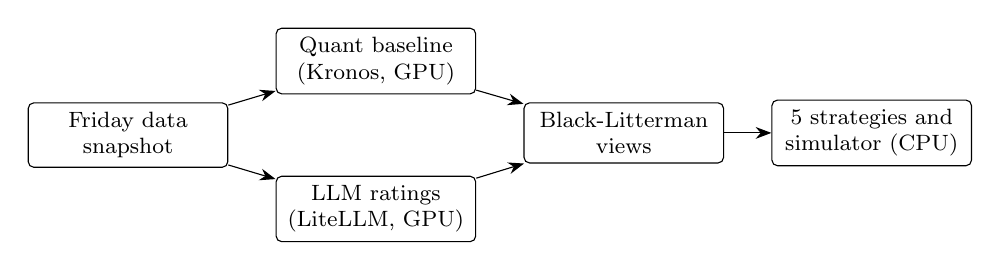
\begin{tikzpicture}[node distance=0.5cm and 0.6cm, every node/.style={draw, rounded corners=2pt, align=center, font=\footnotesize, minimum height=0.75cm, text width=2.3cm}, >={Stealth[length=2mm]}]
\node (d) {Friday data\\snapshot};
\node (k) [above right=0.1cm and 0.6cm of d] {Quant baseline\\(Kronos, GPU)};
\node (l) [below right=0.1cm and 0.6cm of d] {LLM ratings\\(LiteLLM, GPU)};
\node (b) [below right=0.1cm and 0.6cm of k] {Black-Litterman\\views};
\node (s) [right=of b] {5 strategies and\\simulator (CPU)};
\draw[->] (d)--(k); \draw[->] (d)--(l); \draw[->] (k)--(b); \draw[->] (l)--(b); \draw[->] (b)--(s);
\end{tikzpicture}
\caption{The weekly pipeline. The baseline and LLM ratings are computed separately, then combined into views.}
\end{figure}

\textbf{B. Quant baseline:} Each stock is ranked on price momentum and on a five-day return forecast from Kronos, a pretrained forecasting model for price data (102M parameters). Kronos samples 20 possible price paths per stock, and the spread of those paths sets how much weight the baseline view gets.

\textbf{C. LLM ratings:} Each open-weight model rates each stock separately. The model sees the stock's ticker, company name, sector, and that week's news, and it returns a short JSON answer: a low, most likely, and high score on a $-5$ to $5$ scale, plus a one-sentence reason. A narrow range (for example 3 to 5) signals more confidence than a wide one (1 to 5), and the pipeline gives confident views more weight. Every stock is rated under six to seven prompt types: a bare prompt, four to five specialized skills prompts of similar length, and a placebo prompt of the same length with no investing content. All calls use temperature 0.

\textbf{D. Strategies and evaluation:} The ratings are combined with the baseline through Black-Litterman and passed to five fixed strategies: mean-variance, mean-CVaR (which balances return against the average loss in the worst 5\% of outcomes, using 10,000 simulated scenarios), robust mean-variance, resampled mean-variance, and a top-20 portfolio. Each strategy also runs a control portfolio every week that uses the baseline alone, and two more controls (hierarchical risk parity and equal weight) use no forecasts at all. A trade simulator applies the same rules to every portfolio: weekly rebalancing, daily stop-loss and take-profit checks, and a 0.1\% cost per trade. At the end of the study, a permutation test reruns every portfolio 500 times with its scores shuffled across stocks, to show how often random ratings do as well.

\section{Software}
The pipeline uses Python 3.11 with pandas, NumPy, SciPy, scikit-learn, statsmodels, and cvxpy, with PyTorch for Kronos. GPU and CPU jobs run through Slurm. LLM requests use ARCTIC's OpenAI-compatible LiteLLM endpoint, so every open-weight model is called with the same code and settings. I am requesting:
\begin{itemize}
\item \textbf{Existing models:} Gemma 4 31B and MiniMax M2.7, already on the gateway, as the large models.
\item \textbf{New LiteLLM deployments:} Gemma 4 E4B, Phi-4 Mini (3.8B), and Llama 3.2 3B. These small models let the study compare model size and reflect what an ordinary user could run on their own computer.
\item \textbf{Use pattern:} text-only requests, one stock per request, about 2,000 to 8,000 input tokens and 300 output tokens each, sent in a 48-hour weekend window, models in parallel, with no images, tools, or web access. At full scale: about 10,500 requests and 21 to 84 million input tokens per weekend.
\item \textbf{Duration:} all 12 months, with heavy use only in about 24 weekend windows (pilot and live run).
\end{itemize}
One or two small commercial API models (such as Claude Haiku 5.5) are also rated for comparison; they run on their providers' servers and use no ARCTIC compute. All inputs are public market data and published news, with no personal or regulated data. ARCTIC's hosted models are approved for unregulated university data, models banned by GSU's tool registry (such as Qwen) are not used, and papers will disclose AI use.

\section{Justifying Allocation Amounts}
The workload is beyond a single workstation: my own GPU has 6 GB of memory, cannot run Gemma 4 31B or MiniMax M2.7 at all, and would have to run the three small models one after another for every stock and prompt type, leaving little margin before the Monday deadline. The deadline is also why I am requesting an Advanced Research Computing Allocation (ARCA) rather than a startup allocation: Slurm jobs under an ARCA are not preempted, so the weekly Kronos and optimization jobs finish on time.

The estimates below are for the largest planned configuration: 300 stocks, five open-weight models, seven prompt types (bare, placebo, and five skills files), and about 24 weeks of pilot and live runs. Each week that is 300 $\times$ 7 $\times$ 5 = 10,500 LLM requests. Per-request GPU times are given in V100-equivalent seconds. The permutation test covers 250 portfolios (seven models including the commercial ones, seven prompt types, and one baseline control, for each of five strategies), rerun 500 times each: 125,000 replays at an average of about 5 CPU minutes each, with the mean-CVaR and resampled replays the slowest. That is about 12 CPU seconds per portfolio-week, so the weekly run of 252 portfolios needs about 1 CPU hour (listed as 2).

\noindent\begin{minipage}{\linewidth}\centering\setlength{\tabcolsep}{4pt}
\captionof{table}{Estimated ARCTIC usage for the full project.}
\begin{tabular}{lrrrrr}
\toprule
Calculation & Runs/week & Weeks & Time/run & Total SUs & Disk (GB) \\
\midrule
3 small LLMs, ratings & 6,300 & 24 & 10 GPU-sec & 420 GPU & 10 \\
Gemma 4 31B, ratings & 2,100 & 24 & 40 GPU-sec & 560 GPU & 4 \\
MiniMax M2.7, ratings & 2,100 & 24 & 40 GPU-sec & 560 GPU & 4 \\
Kronos forecasts & 1 & 24 & 1 GPU-hour & 24 GPU & 3 \\
Optimization, simulation & 1 & 24 & 2 CPU-hours & 48 CPU & 30 \\
Permutation tests & 125,000 (once) & 1 & 5 CPU-min & 10,420 CPU & 20 \\
Development, testing & n/a & n/a & n/a & 150 GPU, 500 CPU & 15 \\
\midrule
\textbf{Total} & & & & \textbf{1,714 GPU,} \textbf{10,968 CPU} & \textbf{86} \\
\bottomrule
\end{tabular}
\end{minipage}


Table 1 shows my estimated usage: about 1,700 GPU hours, 11,000 CPU hours, and 86 GB of storage. The LLM rows are listed in V100-equivalent GPU hours so the gateway workload can be sized; if LiteLLM usage is accounted separately from Slurm allocations, the GPU hours needed for my own Slurm jobs fall to about 175 (Kronos and development). Storage holds the weekly data snapshots, about 10,500 rating records (about 1 KB each) and 250 portfolio weight files (about 30 KB each) per week, logs, the Kronos weights (about 0.4 GB), the permutation results, and dated backups; it stays on ARCTIC because each week's views use the previous eight weeks of results and the final analysis reruns every week. CPU estimates assume each job uses at most 3 GB of memory per core, so one CPU hour is one SU. To cover failures, retries, and a longer live run, I am requesting \textbf{2,500 GPU hours, 15,000 CPU hours, and 200 GB} for 12 months.

\textbf{Resource use by phase.}
\begin{itemize}
\item \textbf{Development (first 1 to 2 months):} running the full pipeline on each model at the target scale.
\item \textbf{Pilot (1 week):} one full weekend run at the target scale to find problems; it is not counted in the results.
\item \textbf{Live run (about 23 weeks):} one weekend run a week, about 65 GPU and 2 CPU hours each.
\item \textbf{Analysis (final 1 to 2 months):} permutation tests and factor regressions, as parallel CPU jobs.
\end{itemize}
All computation runs on ARCTIC. If the LiteLLM gateway is unavailable during a weekend run, the affected small models are run in my own Slurm GPU jobs instead, which the GPU request above covers. Any week a model still misses is marked and left out of its statistics.
\end{document}
